\chapter{BodyTalk Platform and Game Design}

\begin{figure}[!h]
\centering
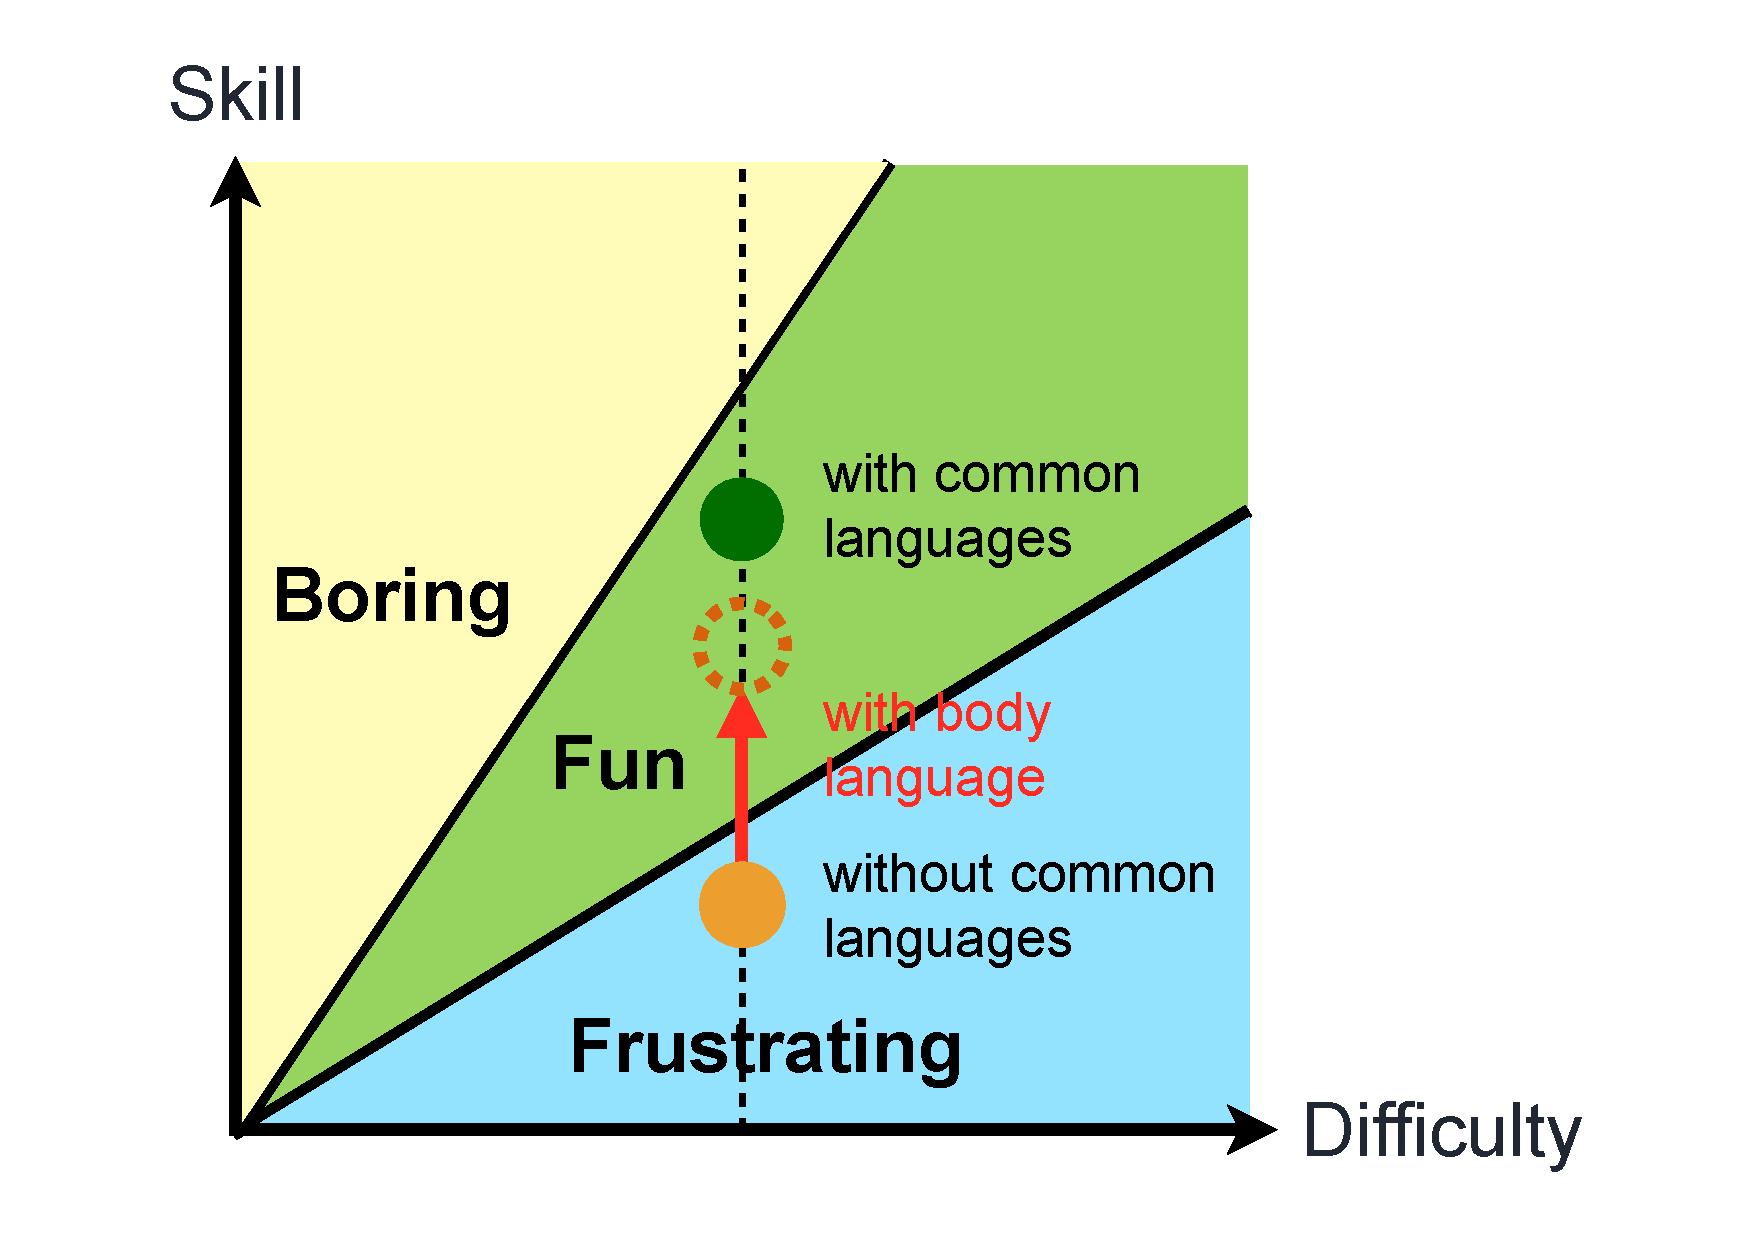
\includegraphics[width=0.9\columnwidth]{Figures/GD_F1.pdf}
\caption{Players cooperative skill levels are lower without a common language. Adding body language communication increases them, and may move the experience from being frustrating to fun.}
\label{fig:GD_F1}
\end{figure}

GameFlow\cite{GD1} discussed how game difficulty and players' skill levels affect whether players would perceive the experience as boring, fun, or frustrating. As shown Figure~\ref{fig:GD_F1}, when the difficulty is greater than the player's skills, the experience is frustrating. On the other hand, when the difficulty is less than the player's skills, the experience will be boring.



Observation from our study indicated that playing a cooperative game with a partner that did not have a common language significantly decreased players' skill level. At a difficulty level that was designed to be fun for players with common languages, that difficulty level was too challenging for players that could not communicate through languages, which lead to a frustrating experience. 

One way to solve this problem is to decrease the game's difficulty. However, this method makes the experience boring for players that had common languages. By adding body language to the gameplay, players without common languages would be able to increase their skill level, and potentially move the experience from frustrating to fun (as shown in Figure~\ref{fig:GD_F1}).  

\section{System Design and Implementation}


Our BodyTalk platform uses a Kinect depth camera (v1) and Micrsoft's Kinect SDK (v1.8) to capture each player's skeletal movement. 
Wii controller is used for navigation (e.g. move left, right, up, down) and selection (e.g. OK, Cancel). 
This combination of input modality enables users to use both arms and both legs freely for expressive body language communication.
These data are sent using Unity engine's\cite{unity} Network View over the Internet in real-time.

We developed a cooperative puzzle platformer game, called Mute Robot, using our BodyTalk platform. Two players at two distinct locations cooperate to solve a series of puzzle challenges, and their body movements are rendered as 3D avatars in real-time (see Figure~\ref{fig:GD_F3}). 


\begin{figure}[!t]
\centering
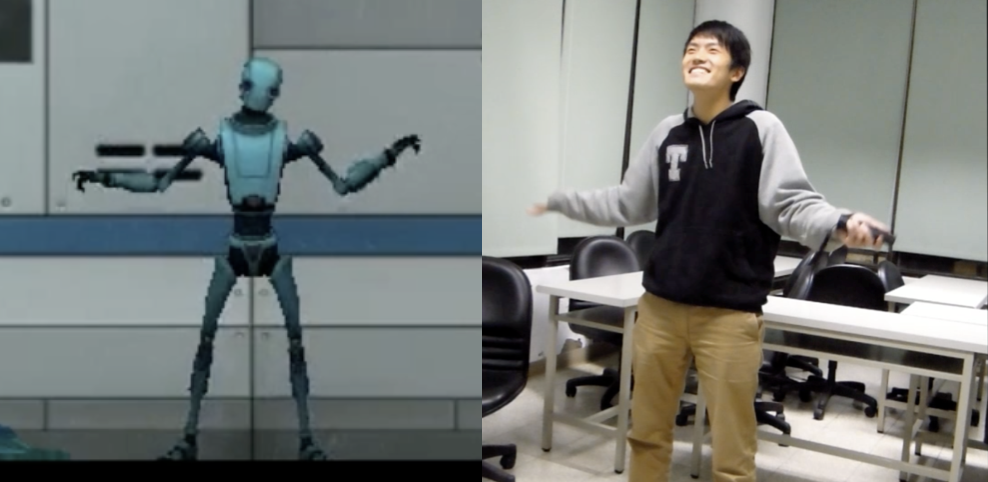
\includegraphics[width=0.9\columnwidth]{Figures/GD_F3.pdf}
\caption{Body movement mapping between player and avatar by Kinect}
\label{fig:GD_F3}
\end{figure}


\begin{figure}[!t]
\centering
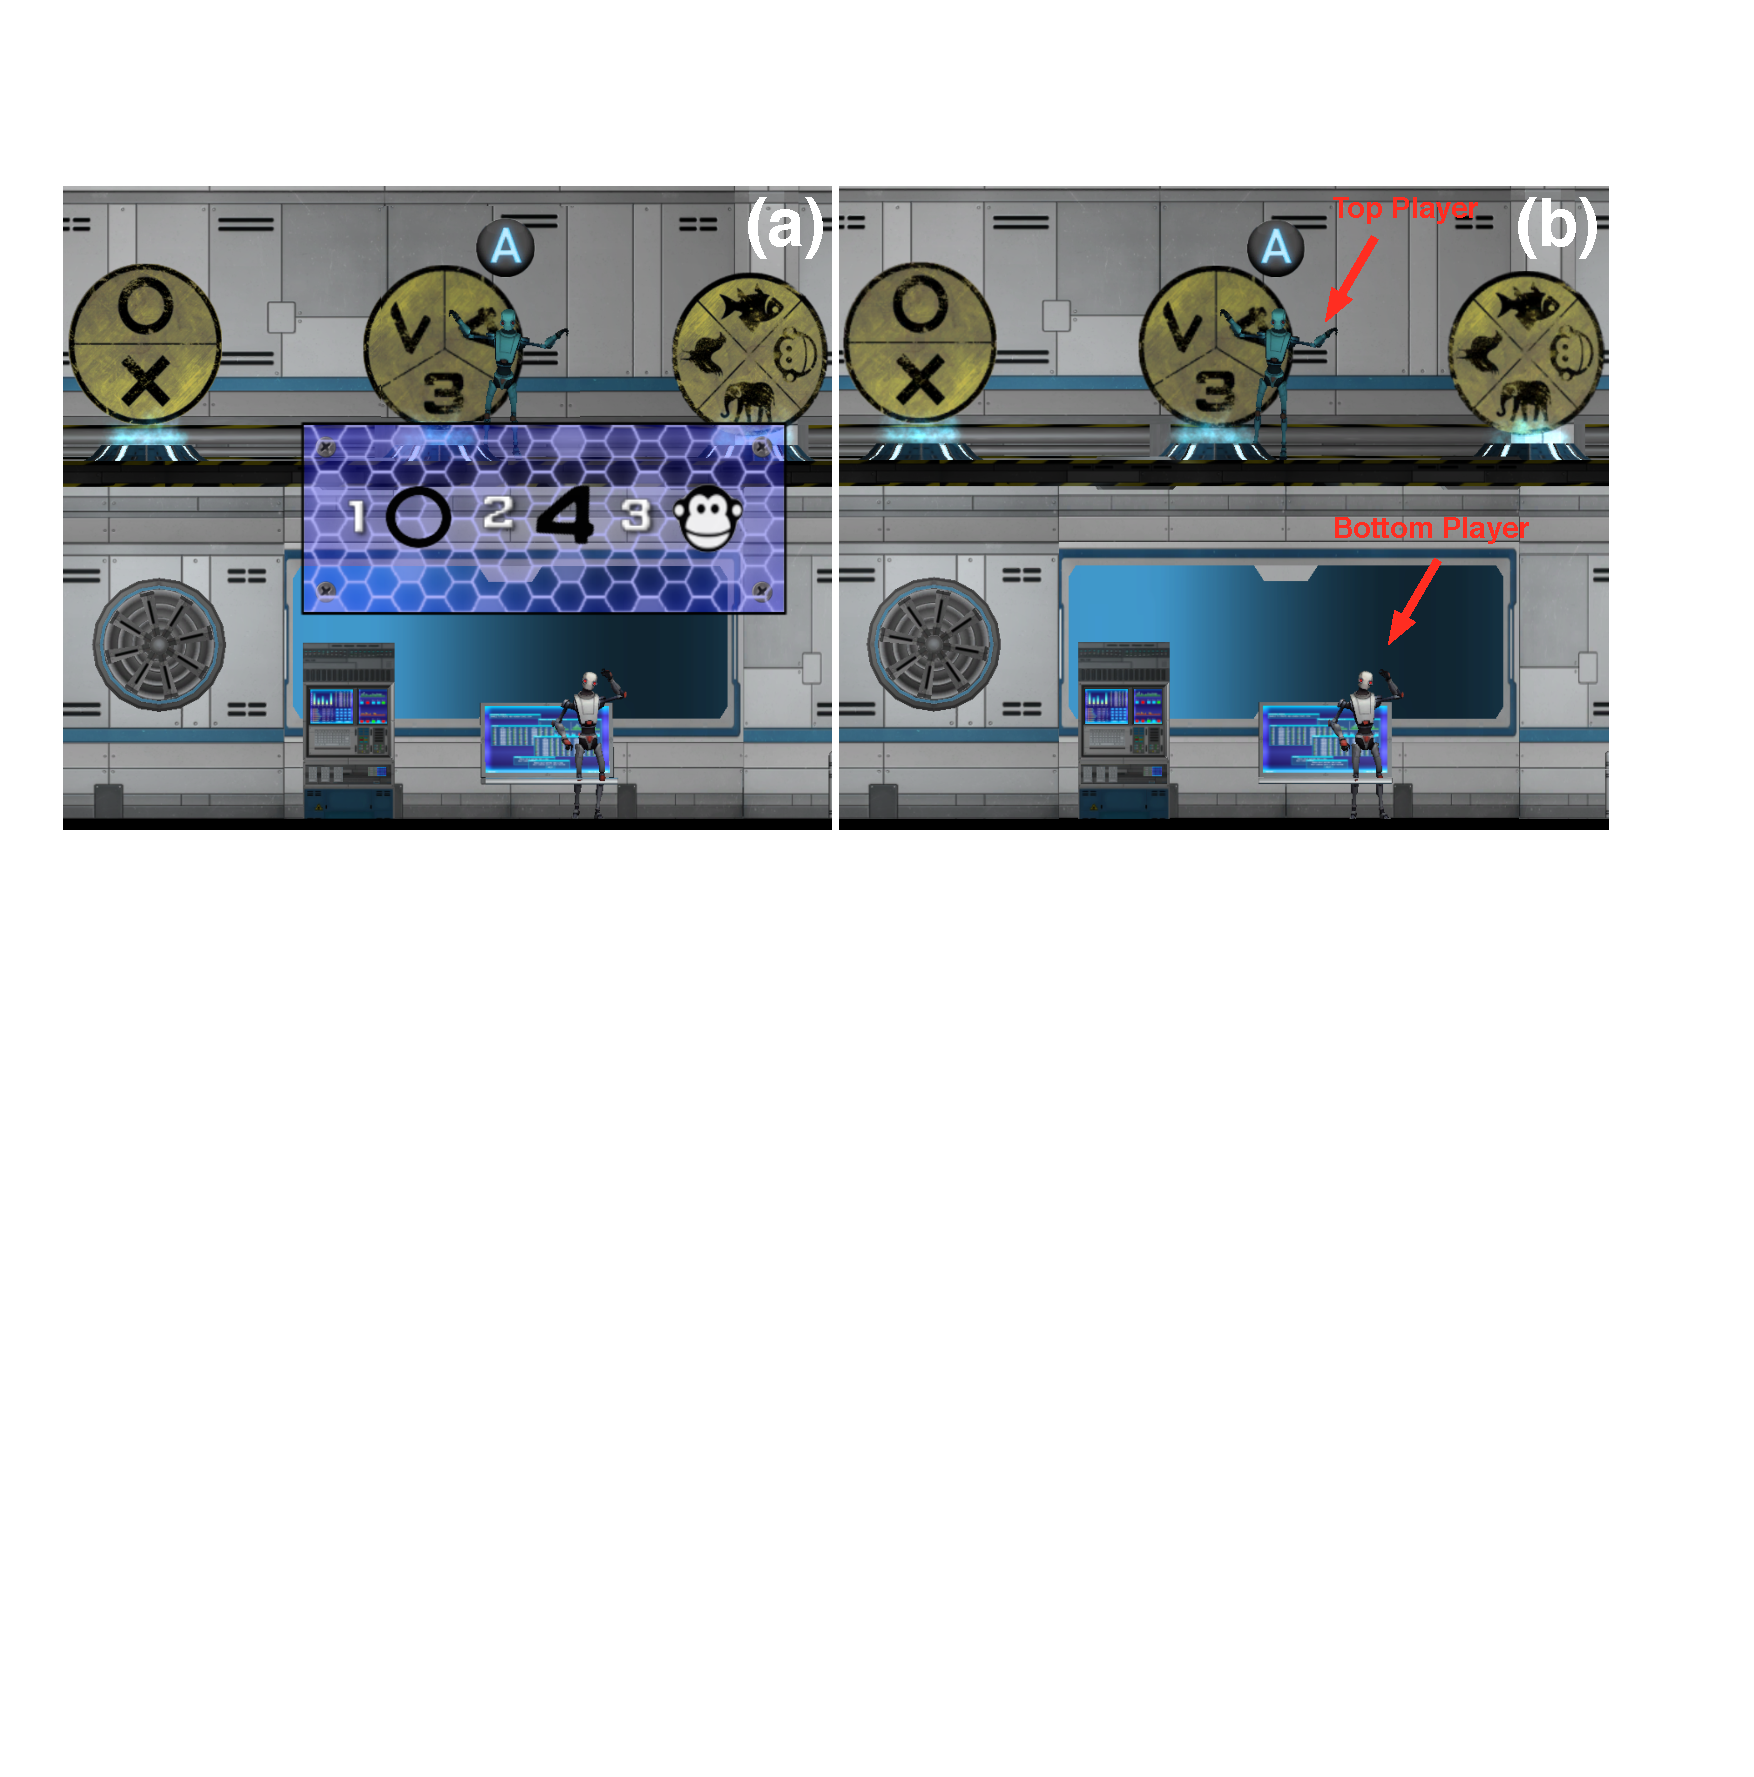
\includegraphics[width=1.0\columnwidth]{Figures/GD_F2.pdf}
\caption{The asymmetric puzzle game design in one of Mute Robot's stages. (a) Bottom player's view, (b) Top player's view}
\label{fig:GD_F2}
\end{figure}


\section{Game Stage Design}


In order to have the players cooperate closely, we designed an asymmetric puzzle gameplay. The two players each sees a different view of the game with only one player receiving the hints to solve a puzzle, and must guide the other player to solve it. The roles of the hint giver and the hint receiver alternate after each stage, and the puzzles increase in difficulty. 

Figure~\ref{fig:GD_F2} shows an example of the two distinct views as seen by the two players. The left view shows the bottom player's view with the puzzle hints, and the right view shows the top player's view (which does not have the hints). 

Our prototype game has three stages. The first stage is a classic puzzle in cooperative games, where one player has to express a randomly generated secret sequence to the other player. In our design, the player must press three spatially separated buttons in the correct order to unlock a door to advance to the next stage.

The second stage, as shown in Figure~\ref{fig:GD_F2}, has a combination lock with three wheels. All three wheels must be turned to the correct selection in order the unlock the door. The first wheel's symbols are two boolean values (O and X). The second wheel's symbols are three numbers (3, 4, 7), and the last wheel's symbols are animals (fish, chicken, monkey and elephant). The set of correct symbols is randomly generated each time.

For the third stage, we wanted to explore abstract concepts. So it randomly selects one of three emotions (angry, happy and tired), for one player to pass to the other player. That player must spell the emotion correctly by selecting from a set of on-screen letters in the correct order to pass the stage.